\chapter{Diseño e implementación} % Main chapter title

\label{Chapter3} % Change X to a consecutive number; for referencing this chapter elsewhere, use \ref{ChapterX}

\definecolor{mygreen}{rgb}{0,0.6,0}
\definecolor{mygray}{rgb}{0.5,0.5,0.5}
\definecolor{mymauve}{rgb}{0.58,0,0.82}

%%%%%%%%%%%%%%%%%%%%%%%%%%%%%%%%%%%%%%%%%%%%%%%%%%%%%%%%%%%%%%%%%%%%%%%%%%%%%
% parámetros para configurar el formato del código en los entornos lstlisting
%%%%%%%%%%%%%%%%%%%%%%%%%%%%%%%%%%%%%%%%%%%%%%%%%%%%%%%%%%%%%%%%%%%%%%%%%%%%%
\lstset{ %
  backgroundcolor=\color{white},   % choose the background color; you must add \usepackage{color} or \usepackage{xcolor}
  basicstyle=\footnotesize,        % the size of the fonts that are used for the code
  breakatwhitespace=false,         % sets if automatic breaks should only happen at whitespace
  breaklines=true,                 % sets automatic line breaking
  captionpos=b,                    % sets the caption-position to bottom
  commentstyle=\color{mygreen},    % comment style
  deletekeywords={...},            % if you want to delete keywords from the given language
  %escapeinside={\%*}{*)},          % if you want to add LaTeX within your code
  %extendedchars=true,              % lets you use non-ASCII characters; for 8-bits encodings only, does not work with UTF-8
  %frame=single,	                % adds a frame around the code
  keepspaces=true,                 % keeps spaces in text, useful for keeping indentation of code (possibly needs columns=flexible)
  keywordstyle=\color{blue},       % keyword style
  language=[ANSI]C,                % the language of the code
  %otherkeywords={*,...},           % if you want to add more keywords to the set
  numbers=left,                    % where to put the line-numbers; possible values are (none, left, right)
  numbersep=5pt,                   % how far the line-numbers are from the code
  numberstyle=\tiny\color{mygray}, % the style that is used for the line-numbers
  rulecolor=\color{black},         % if not set, the frame-color may be changed on line-breaks within not-black text (e.g. comments (green here))
  showspaces=false,                % show spaces everywhere adding particular underscores; it overrides 'showstringspaces'
  showstringspaces=false,          % underline spaces within strings only
  showtabs=false,                  % show tabs within strings adding particular underscores
  stepnumber=1,                    % the step between two line-numbers. If it's 1, each line will be numbered
  stringstyle=\color{mymauve},     % string literal style
  tabsize=2,	                   % sets default tabsize to 2 spaces
  title=\lstname,                  % show the filename of files included with \lstinputlisting; also try caption instead of title
  morecomment=[s]{/*}{*/}
}


%----------------------------------------------------------------------------------------
%	Chapter 3
%----------------------------------------------------------------------------------------

En este capítulo se realiza una explicación detallada del diseño del hardware, cómo se utilizó cada componente principal y su conexión con el microcontrolador. Asimismo, se especifica la estructura general del firmware en el marco de FreeRTOS y las principales rutinas de bajo nivel.


\section{Arquitectura de hardware}

La arquitectura general de la placa fue diseñada para tener como unidad de procesamiento principal al microcontrolador STM32 de la placa NUCLEO-144 y a la pantalla LCD como periférico principal de salida de datos.

La figura \ref{fig:estrucInt} muestra un diagrama completo de todo el hardware de la placa fabricada, sus entradas, salidas y el conexionado entre sus distintas partes. También incluye los periféricos utilizados en el microcontrolador y la cantidad de líneas de cada conexión.

\begin{figure}[H]
\centering
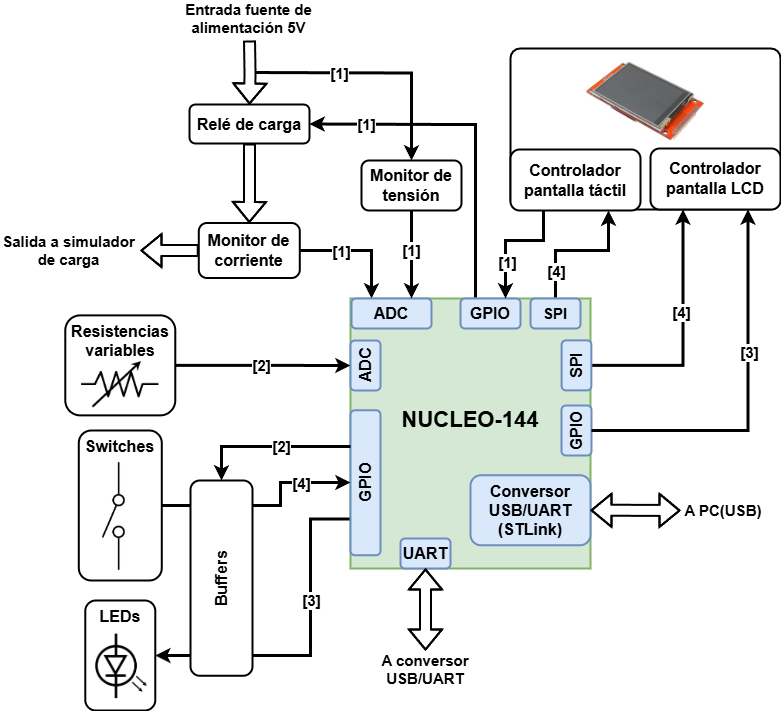
\includegraphics[width=0.84\textwidth]{./Figures/diagDisp.png}
\caption{Diagrama completo del hardware implementado.}
\label{fig:estrucInt}
\end{figure}

Todos los bloques externos a la placa NUCLEO que se ven en el diagrama, a excepción de la pantalla LCD, fueron diseñados con componentes electrónicos básicos, es decir, sin usar módulos funcionales compactos.

Los bloques internos de la placa NUCLEO que se ven en el diagrama, a excepción del conversor USB-UART, son periféricos que se encuentran embebidos en el mismo chip del microcontrolador. El conversor USB-UART, denominado STLink, se encuentra fuera de este y esta compuesto por varios componentes electrónicos.

En el apéndice \ref{AppendixA} se encuentra el diseño esquemático completo de la placa.

\subsection{Medición de corriente del amplificador}

El principio de funcionamiento del monitor de corriente se basa en un resistor \textit{shunt}, el cual se coloca sobre la alimentación, en serie con la línea a la que se desea conocer el consumo de corriente. Para que este resistor no disipe mucha potencia y disminuya la tensión de la línea, su valor de resistencia es de 10 \si{m\ohm}. Mientras menos comparable sea su valor al de la carga más despreciables serán los efectos negativos que introducirá.

Sobre este resistor cae una tensión proporcional a la corriente consumida por el EDFA. Como el valor máximo de corriente consumida por el amplificador se encuentra cerca de los 2,5 A, sobre el resistor caen como máximo 25 mV, lo que frente a los 5 V de la alimentación no representa un valor significativo. Luego de sensarla, el chip amplifica 100 veces esta tensión diferencial y la conecta a uno de sus pines de salida.

Al ser este un valor analógico, para poder ser interpretado se lo debe convertir a digital. Para esto se usa el ADC incorporado en el microcontrolador, conectando a uno de sus pines la señal de salida del monitor de corriente. La tensión máxima que puede alcanzar la señal es de aproximadamente 2,5 V, lo que se encuentra por debajo de la tensión de referencia del ADC. Un esquema de esta conexión se puede ver en la figura \ref{fig:funcMonitor}.

\begin{figure}[H]
\centering
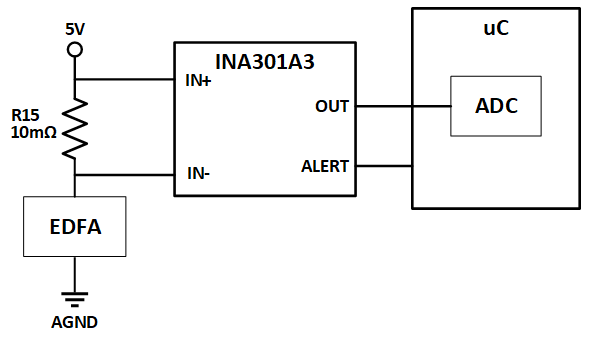
\includegraphics[width=0.75\textwidth]{./Figures/func_monitor.png}
\caption{Esquema del monitor de corriente.}
\label{fig:funcMonitor}
\end{figure}

Por otro lado, el INA301A3 cuenta con un pin de salida denominado ALERT que se activa cuando la corriente medida alcanza cierto valor, lo que funciona a modo de alarma. Este nivel se determina conectando un resistor de cierto valor en el pin LIMIT.

\subsection{Relé de alimentación}

La línea de 5 V de alimentación del EDFA es controlada mediante la activación de un relé (código APAN3103) \citep{WEBSITE:RELE_DS}, lo que significa que la conexión y desconexión es mecánica. Esto se decidió implementarlo así debido a los lineamientos de protecciones necesarios para el hardware de vuelo.

Como el relé necesita de aproximadamente 36,7 mA para activarse, no se puede conectar directamente a un pin de salida del microcontrolador ya que este no puede suministrar la corriente necesaria. Por esta razón la activación se realiza mediante un transistor (código MMBT2222) \citep{WEBSITE:TRANS_DS}, funcionando como una llave (en modo saturación o corte). De esta forma, la corriente para la activación de la bobina del relé la provee directamente la fuente de alimentación de 3,3 V.

\subsection{Medición de tensión del amplificador}

Hacer una medición de la tensión de la línea es mucho más sencillo que hacer una medición de la corriente, ya que esta se puede conectar directamente a un ADC si previamente se la atenúa o amplifica (dependiendo del caso).

En este caso, como la tensión de alimentación del EDFA es 5 V y la tensión de referencia del ADC del microcontrolador es 3,3 V, se la debe atenuar de forma que esta se encuentre dentro del fondo de escala del ADC.

Considerando que se desea medir una sobretensión de por lo menos 1 V en la alimentación, se opta por atenuar la tensión del EDFA a la mitad, resultando en un fondo de escala de 6,6 V.

Esta técnica permite medir tensiones mayores a la de referencia del ADC pero trae como desventaja que se pierde precisión debido al ruido y la tolerancia de los resistores.

En la figura \ref{fig:monTension} se puede ver el circuito implementado.

\begin{figure}[H]
\centering
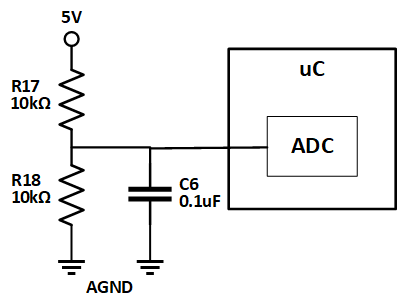
\includegraphics[width=0.5\textwidth]{./Figures/mon_tension.png}
\caption{Circuito del monitor de corriente.}
\label{fig:monTension}
\end{figure}

El capacitor C6 forma un filtro RC \citep{WEBSITE:RC_CIRCUIT} para eliminar el ruido de alta frecuencia que pueda tener la línea.

\subsection{Conexión a pantalla LCD}
\label{sec:conLCD}

Como se puede ver en la figura \ref{fig:estrucInt}, la pantalla LCD tiene dos controladores con SPI: uno para el control de la pantalla y otro para el control de la función táctil. Si bien ambas interfaces se podrían haber conectado al mismo periférico SPI del microcontrolador en modo multi-esclavo, se decidió usar uno para cada uno de forma individual. La principal razón de esto es porque facilita la implementación del firmware ya que permite usar ambos controladores de forma independiente y a distintas velocidades sin necesidad de reconfiguración.

El controlador de la función táctil tiene, además de las señales del bus SPI, una señal denominada IRQ que se activa cuando se detecta que la pantalla está siendo tocada. Esta señal sirve para ser usada como interrupción en el programa del microcontrolador.

Por otro lado, el controlador del display también tiene señales con funciones especiales. Estas son:

\begin{itemize}
\item RESET: resetea el chip del controlador y, por lo tanto, toda la configuración del display y la información de cada píxel.
\item DC/RS: indica al controlador si la información que se está enviando por el SPI es un dato o un registro, dependiendo del nivel de la señal.
\item LED: permite controlar la intensidad de luz de la pantalla (denominada \textit{backlight}).
\end{itemize}

\subsection{Entradas y salidas digitales}

En la tabla \ref{tab:señalesConector} se detallan las señales de entrada y salida digitales del puerto del EDFA. Las salidas son señales de alarmas y las de entrada, de control.

Estas señales se podrían conectar directamente a pines digitales del microcontrolador ya que son de tipo TTL 3,3 V, pero se decidió poner antes de este un \textit{buffer} de tres estados (código SN74LVC2244A) \citep{WEBSITE:BUFFERS_DS}. Los objetivos de esta decisión son tres:

\begin{itemize}
\item Generar niveles de tensión mejor definidos. Esto filtra ruido y rebote en las señales y facilita la detección en ambos extremos (EDFA y microcontrolador).
\item Proveer a la electrónica interna del EDFA de protección contra descargas electrostáticas (ESD).
\item Suministrar la corriente necesaria a las señales de entrada del amplificador y así evitar que esta deba ser proporcionada por el microcontrolador.
\end{itemize}

Para poder simular la activación de las alarmas en la placa se colocaron pulsadores con testigo lumínico (código TL1265YQSCLR) \citep{WEBSITE:PULSADOR_DS} en el extremo donde estaría el EDFA, con el propósito de activarlos manualmente durante el testeo del firmware.

Para las señales de control se utilizaron LEDs que indican el estado de activación de estas (código AA3528LVBS/D) \citep{WEBSITE:LEDS_DS}.

\subsection{Indicadores de potencia óptica}

Las señales IN\_POW y OUT\_POW son analógicas y pueden tomar cualquier valor en el rango de 0 V a 3,3 V. Este valor es proporcional a la potencia óptica medida por los detectores de entrada y salida del amplificador, el cual corresponde al rango de -10 dBm a 10 dBm para el de entrada y 5 dBm a 37 dBm para el de salida.

Para poder simular estas señales se utilizaron dos resistores variables (código PTV09A-4020U-B103) \citep{WEBSITE:POTENC_DS} que permiten variar de forma manual el valor de tensión entre 0 V y 3,3 V.

\subsection{Interfaz UART}

Como se puede ver en la figura \ref{fig:estrucInt}, el dispositivo debe contar con dos interfaces UART: una para la comunicación entre el tester y el EDFA y otra para la comunicación entre el tester y la PC. Para esto se requiere hacer uso de dos de los controladores UART internos que posee el microcontrolador.

\section{Arquitectura de firmware}

Como se mencionó anteriormente, la arquitectura del firmware del trabajo tiene como base la utilización de FreeRTOS y los recursos que ofrece. Esto permite la implementación de un diseño eficaz y sencillo mediante la división en dos partes bien definidas: la parte de procesamiento de datos y control (o backend) y la parte gráfica que interactúa con el usuario (o frontend). Para implementar cada una de ellas se utilizó una tarea o proceso, recurso provisto por el sistema operativo. Como la velocidad de reloj del microcontrolador es alta, se puede asumir que estas se ejecutan de forma independiente y simultánea. Por otro lado, estas comparten ciertas variables cuyo acceso debe ser controlado para que no existan colisiones de lectura o escritura. Este acceso es gestionado por un semáforo.

El proceso del backend tiene como tarea principal ejecutar una máquina de estados y se encarga de controlar el estado general del dispositivo en todo momento. Esto significa que lee los datos de entrada, los procesa y en base a ellos toma decisiones que terminan por afectar las señales de salida y en última instancia a la tarea del display.

Por otro lado, el proceso del frontend esta asociado al display LCD y tiene como objetivo principal la interacción directa con el usuario. Para ello, debe leer la información de salida del backend, presentarla en la pantalla y, a su vez, detectar cuándo y dónde el usuario presiona sobre ella y enviar estos datos al backend mediante recursos compartidos. 

En la figura \ref{fig:arqFW} se puede ver un diagrama de cómo se relacionan ambas tareas entre sí y con el hardware.

\begin{figure}[H]
\centering
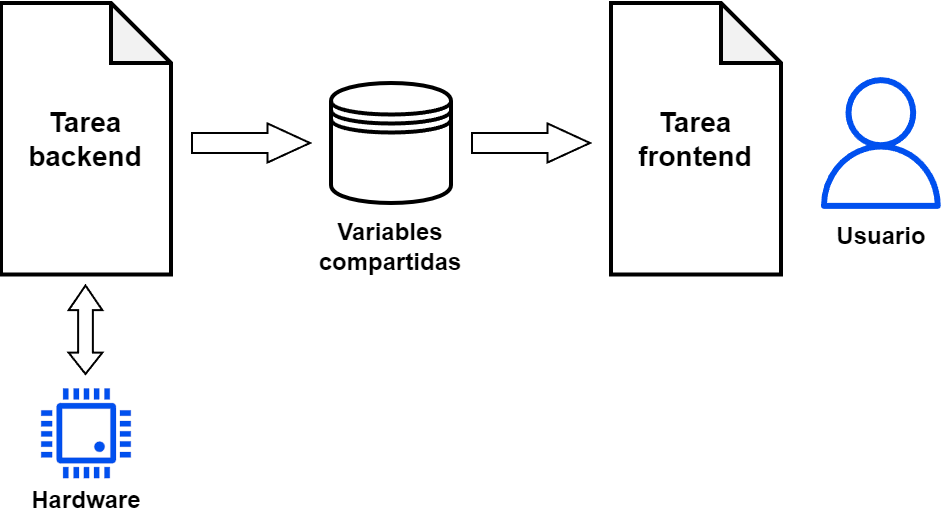
\includegraphics[width=0.85\textwidth]{./Figures/arqFW.png}
\caption{Arquitectura de firmware.}
\label{fig:arqFW}
\end{figure}

\subsection{Tarea del frontend}



\begin{figure}[H]
\centering
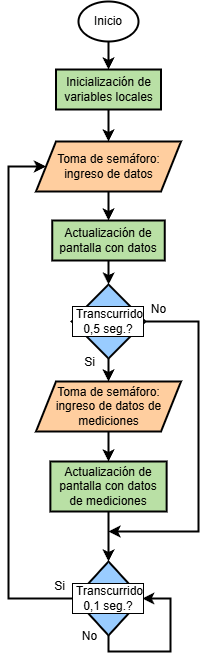
\includegraphics[width=0.4\textwidth]{./Figures/flowTaskDisp.png}
\caption{Diagrama de flujo de la tarea del frontend.}
\label{fig:taskDisp}
\end{figure}

\subsection{Tarea del backend}



%\begin{figure}[H]
%\centering
%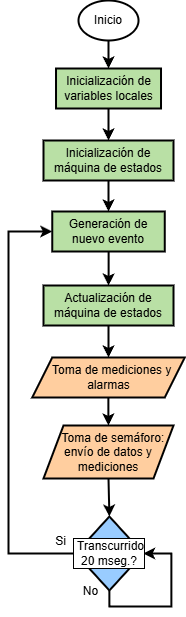
\includegraphics[width=0.4\textwidth]{./Figures/flowTaskApp.png}
%\caption{Diagrama de flujo de la tarea del backend.}
%\label{fig:taskApp}
%\end{figure}

\subsection{Máquina de estados}
\subsubsection{Diseño}

La máquina de estados implementada administra el funcionamiento del amplificador en todo momento mediante su interfaz eléctrica y el control de la alimentación. Cada uno de los estados de la máquina describen de forma análoga el estado real del EDFA. En base a los requerimientos se han definido los siguientes:

\begin{itemize}
\item Desconectado: alimentación del amplificador desconectada (relé desactivado y valor de tensión válido).
\item Conectado: amplificador energizado (relé activado).
\item Activo: salida óptica del amplificador encendida.
\item Alimentación fuera de rango: valor de la alimentación del EDFA fuera del rango permitido.
\item Alarma encendida: alarma del EDFA encendida (cualquiera de ellas).
\end{itemize}

Todas las posibles transiciones entre estos estados son disparadas por eventos que pueden ocurrir en cualquier momento, y ejecutan una acción según el estado en que se encuentre la máquina. La cantidad de eventos que pueden llegar a la máquina es elevada, por lo que, por simplicidad solo se mencionan algunos a modo de ejemplo:

\begin{itemize}
\item Eventos de la alimentación: baja tensión, sobretensión y sobrecorriente.
\item Eventos de la pantalla táctil: botón de encendido presionado, botón de apagado presionado, etc.
\item Eventos del amplificador: alarma de potencia de entrada encendida, potencia óptica de salida excedida, etc.
\item Eventos de la consola de control: comando de conexión de alimentación recibido, comando de encendido de salida del amplificador recibido, comando inválido, etc.
\end{itemize}

En la figura \ref{fig:diagFSM} se puede ver un diagrama simplificado de transiciones de la máquina de estados implementada, que incluye sus estados y eventos asociados.

\begin{figure}[H]
\centering
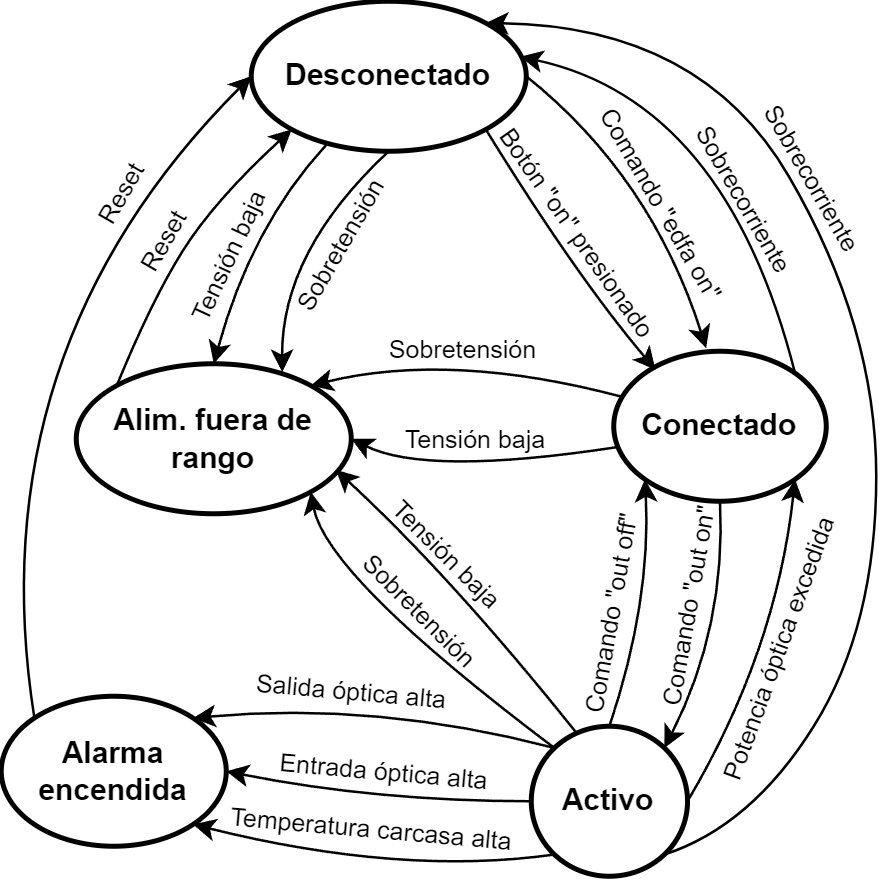
\includegraphics[width=0.9\textwidth]{./Figures/diagFSM.png}
\caption{Diagrama simplificado de la máquina de estados.}
\label{fig:diagFSM}
\end{figure}

\subsubsection{Implementación}

%\begin{figure}[H]
%\centering
%\includegraphics[width=0.9\textwidth]{./Figures/typesFSM.png}
%\caption{Tipos de datos de la FSM.}
%\label{fig:typesFSM}
%\end{figure}

\subsection{Capa de abstracción del amplificador}

Con el objetivo de generar una estructura jerárquica, se decidió crear una capa adicional que se ubica por encima de los drivers de la pantalla LCD, de la pantalla táctil, de la UART, de las señales analógicas y de los GPIO provistos por la HAL del fabricante (ST). A su vez, los drivers de la pantalla LCD y la pantalla táctil se implementan con base en el driver de SPI, ya que debe hacer uso de las funciones de bajo nivel para el envío y recepción de datos y comandos. Para el ADC también se creó una pequeña capa superior que permite obtener todos los valores de las señales analógicas en formato de punto flotante.

De esta forma se genera un nivel más de abstracción que provee un conjunto de funciones o servicios para interactuar con el EDFA, funcionando a modo de puente entre este y la aplicación de usuario (backend). En la figura \ref{fig:halAmp} se puede ver la estructura de esta capa junto con sus distintos niveles.

\begin{figure}[H]
\centering
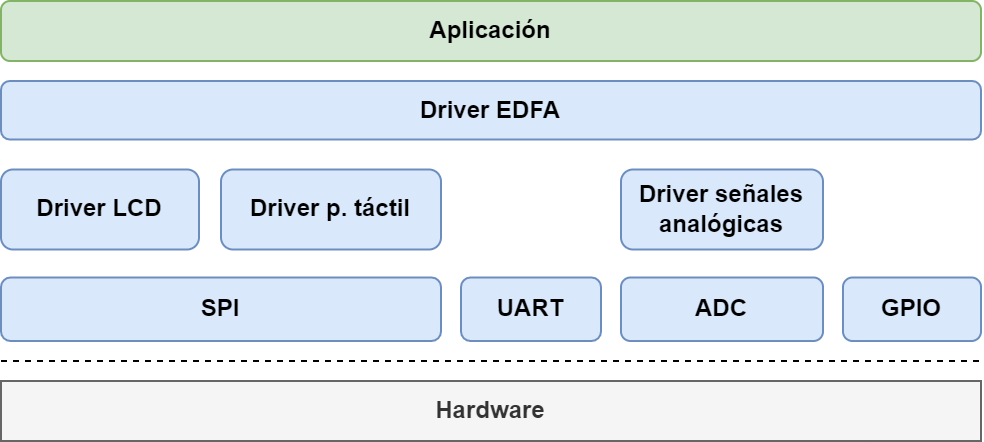
\includegraphics[width=0.9\textwidth]{./Figures/halamp2.png}
\caption{Capa de abstracción del EDFA.}
\label{fig:halAmp}
\end{figure}

\subsection{Driver del ADC}

Para la lectura de los valores analógicos se decidió utilizar el driver del ADC mediante DMA. Esto trae la principal ventaja de que solo se necesita realizar la configuración del ADC una sola vez al comienzo del programa y luego el muestreo y la conversión de los valores se realizará automáticamente de forma periódica.

En este caso esta implementación es particularmente útil debido a que se evita ocupar al procesador realizando la conversión manualmente y se puede atender a otras tareas. De esta forma, como el movimiento del dato convertido desde el periférico a la memoria se hace de forma automática, cuando el programa requiere leer el dato del valor convertido este ya se encuentra disponible en memoria.

Para filtrar ruido y posibles valores espurios que tome la señal analógica se aplica un pequeño filtro promediando 10 muestras continuas en cada canal usado. La configuración completa del ADC se muestra en la tabla \ref{tab:configADC}.

\begin{table}[H]
	\centering
	\caption{Configuración del ADC.}
	\begin{tabular}{l c}
		\toprule
		\textbf{Parámetro} & \textbf{Configuración}  \\
		\midrule
		Cantidad de canales usados & 4		\\
		Cantidad de bits		& 12 bits 	 		 \\
		Modo de conversión		& Continua   \\
		Tasa de muestreo		& 600 ksps	 \\
		Cantidad de muestras promediadas	& 10 \\
		Disparo de conversión	& Por software \\
		\bottomrule
		\hline
	\end{tabular}
	\label{tab:configADC}
\end{table}

Dado que el ADC opera con 12 bits y la tensión de referencia del microcontrolador es de 3,3 V, se obtienen 4096 niveles discretos (de 0 a 4095), lo que resulta en una resolución de aproximadamente 0,8 mV por cada bit menos significativo.

\subsection{Driver de la pantalla LCD}

Como se mencionó en la sección \ref{sec:conLCD}, cada bus SPI (LCD y pantalla táctil) tiene una interfaz dedicada en el microcontrolador funcionando este en modo maestro. La tabla \ref{tab:configSPI} muestra un resumen de la configuración de ambos controladores.

\begin{table}[H]
	\centering
	\caption{Configuración de los SPI del LCD.}
	\begin{tabular}{l c c}
		\toprule
		\textbf{Parámetro} & \textbf{LCD} & \textbf{Pantalla táctil} \\
		\midrule
		Velocidad de transmisión	& 8 Mbps & 4 Mbps	\\
		Ancho de palabra 				& 8 bits & 8 bits	    \\
		Polaridad							& Baja & Baja \\
		Dirección							& Bidireccional & Bidireccional \\
		\bottomrule
		\hline
	\end{tabular}
	\label{tab:configSPI}
\end{table}

Debido a la cantidad de píxeles de la pantalla LCD y el tiempo que le toma al programa actualizarla en su totalidad, se decidió actualizarla a una tasa de diez veces por segundo. Teniendo en cuenta que en esta aplicación los eventos visibles ocurren a baja velocidad, aumentar la tasa de muestreo no aportaría una mejora significativa. En cuanto a las variables, para poder ser legibles, sus valores se actualizan solamente dos veces por segundo.

\subsection{Driver de UART}

El controlador de UART para ambas interfaces se configura de modo que genere una interrupción en el programa luego de recibir una cadena de caracteres. Esto funciona de forma que los caracteres que se reciben se guardan continuamente en un buffer de entrada hasta que la línea de datos pasa a estar inactiva. Luego se atiende la interrupción y en ella se copia al programa principal la cadena de caracteres del buffer para ser analizada.

En la tabla \ref{tab:configUART} se puede ver la configuración de ambas interfaces UART.

\begin{table}[H]
	\centering
	\caption{Configuración de la interfaz UART.}
	\begin{tabular}{l c}
		\toprule
		\textbf{Parámetro} & \textbf{Configuración} \\
		\midrule
		Velocidad de transmisión	& 115200 baudios \\
		Ancho de palabra 				& 8 bits \\
		Bits de stop						& 1 bit \\
		Paridad							    & Ninguna \\
		Control de hardware			& Ninguno \\
		\bottomrule
		\hline
	\end{tabular}
	\label{tab:configUART}
\end{table}

\subsection{Consola de control}

%habria que mencionar en alguno de las primeras secciones la existencia de la consola de control

La consola de control brinda una pequeña interfaz que funciona como intermediario entre el usuario y el amplificador, permitiéndole consultar y controlar su estado en todo momento. También se utiliza para ingresar valores al dispositivo, tales como los niveles de tensión y corriente máximos admitidos.

La consola corre sobre la tarea del backend y puede inyectar eventos a la máquina de estados. Su funcionamiento es similar al de cualquier consola, usando un esquema de comando y argumento. La tabla \ref{tab:tablacmd} lista todos los pares comando/argumento que puede recibir la consola.

\begin{table}[H]
	\centering
	\caption{Comandos/argumentos de la consola.}
	\begin{tabular}{l c p{8cm}}
		\toprule
		\textbf{Comando} & \textbf{Argumento} & \textbf{Descripción} \\
		\midrule
		edfa	& on & Conecta la alimentación del EDFA.	\\
		edfa	& off & Desconecta la alimentación del EDFA. \\
		out	& on & Prende la salida óptica del EDFA. \\
		out   & off & Apaga la salida óptica del EDFA. \\
		status & - & Indica el estado general del EDFA y los valores de las variables. \\
		reset & - & Envía la señal de reset al microcontrolador del EDFA. \\
		ilim	& (valor) & Establece el límite de corriente al valor del argumento. \\
		vul	& (valor) & Establece el límite superior de tensión al valor del argumento. \\
		vll		& (valor) & Establece el límite inferior de tensión al valor del argumento. \\
		oipl	& (valor) & Establece el límite de potencia de entrada al valor del argumento. \\
		oopl & (valor) & Establece el límite de potencia de salida al valor del argumento. \\
		\bottomrule
		\hline
	\end{tabular}
	\label{tab:tablacmd}
\end{table}

\section{Dispositivo implementado}
\label{sec:dispImp}

Es importante aclarar que el dispositivo que se desarrolló e integró como solución a lo planteado en el capítulo 1 no es el producto final destinado a ser utilizado. La placa construida se puede interpretar como un prototipo de desarrollo o una versión de ingeniería, ya que cumple con dos objetivos principales: verificar el funcionamiento del hardware diseñado y desarrollar el firmware que se ejecutará en el microcontrolador. 

La versión armada para este trabajo, incluye los mismos componentes previstos para el producto final y, además, incorpora el hardware necesario para emular la interfaz electrónica del modelo del amplificador óptico, lo que permite generar todas las señales del conector, tanto analógicas como digitales.

Una vez alcanzados estos objetivos, la siguiente etapa consiste en desarrollar la placa del producto final, con el factor de forma adecuado para integrar y montar todos los componentes en una carcasa transportable. 

El PCB fue enviado a fabricar a la empresa china JLCPCB y consta de 4 capas: dos planos internos de referencia conectados a 3,3 V y GND y dos capas de señal (\textit{Top} y \textit{Bottom}). En la figura \ref{fig:placa1} y \ref{fig:placa2} se pueden ver dos fotos del PCB ensamblado sin el display ni la placa NUCLEO conectados (lado superior y lado inferior respectivamente). Por último, en la figura \ref{fig:placa3} se puede ver la placa con ambos módulos conectados.

\begin{figure}[H]
     \centering
     \begin{subfigure}{\textwidth}
         \centering
         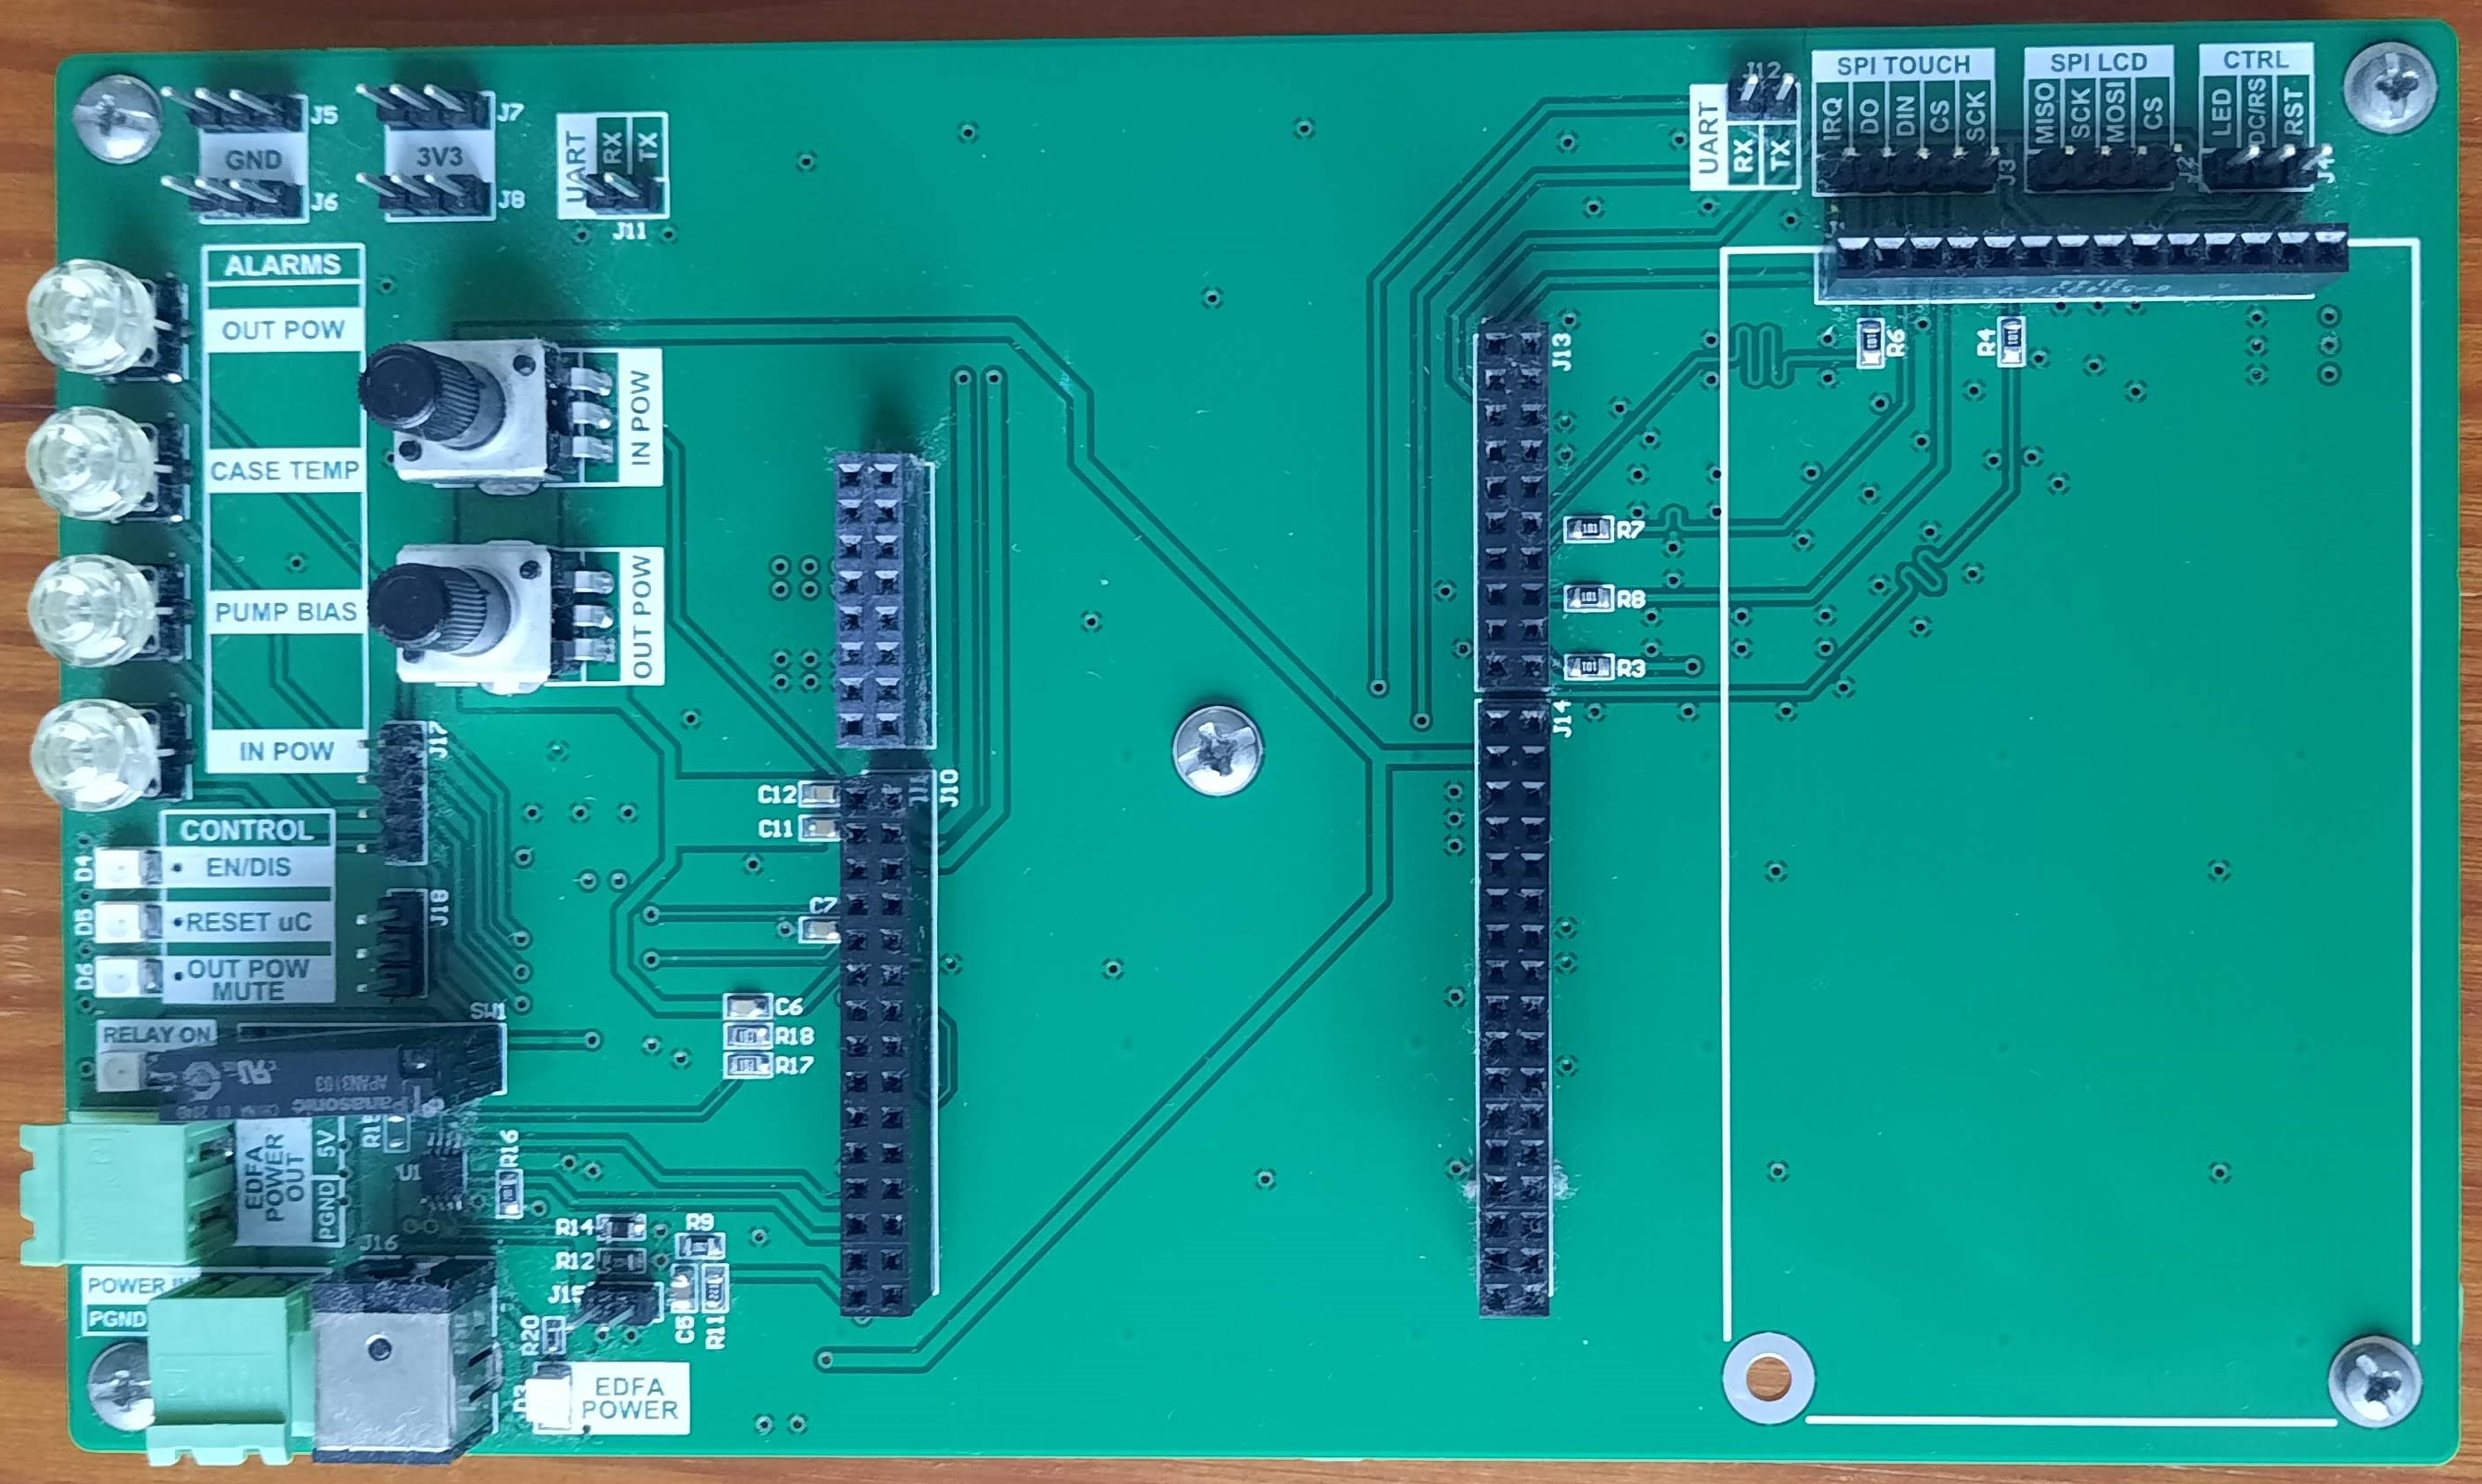
\includegraphics[width=.75\textwidth]{./Figures/placa2.jpg}
         \caption{Lado superior del PCB.}
         \label{fig:placa1}
     \end{subfigure}
     \begin{subfigure}{\textwidth}
         \centering
         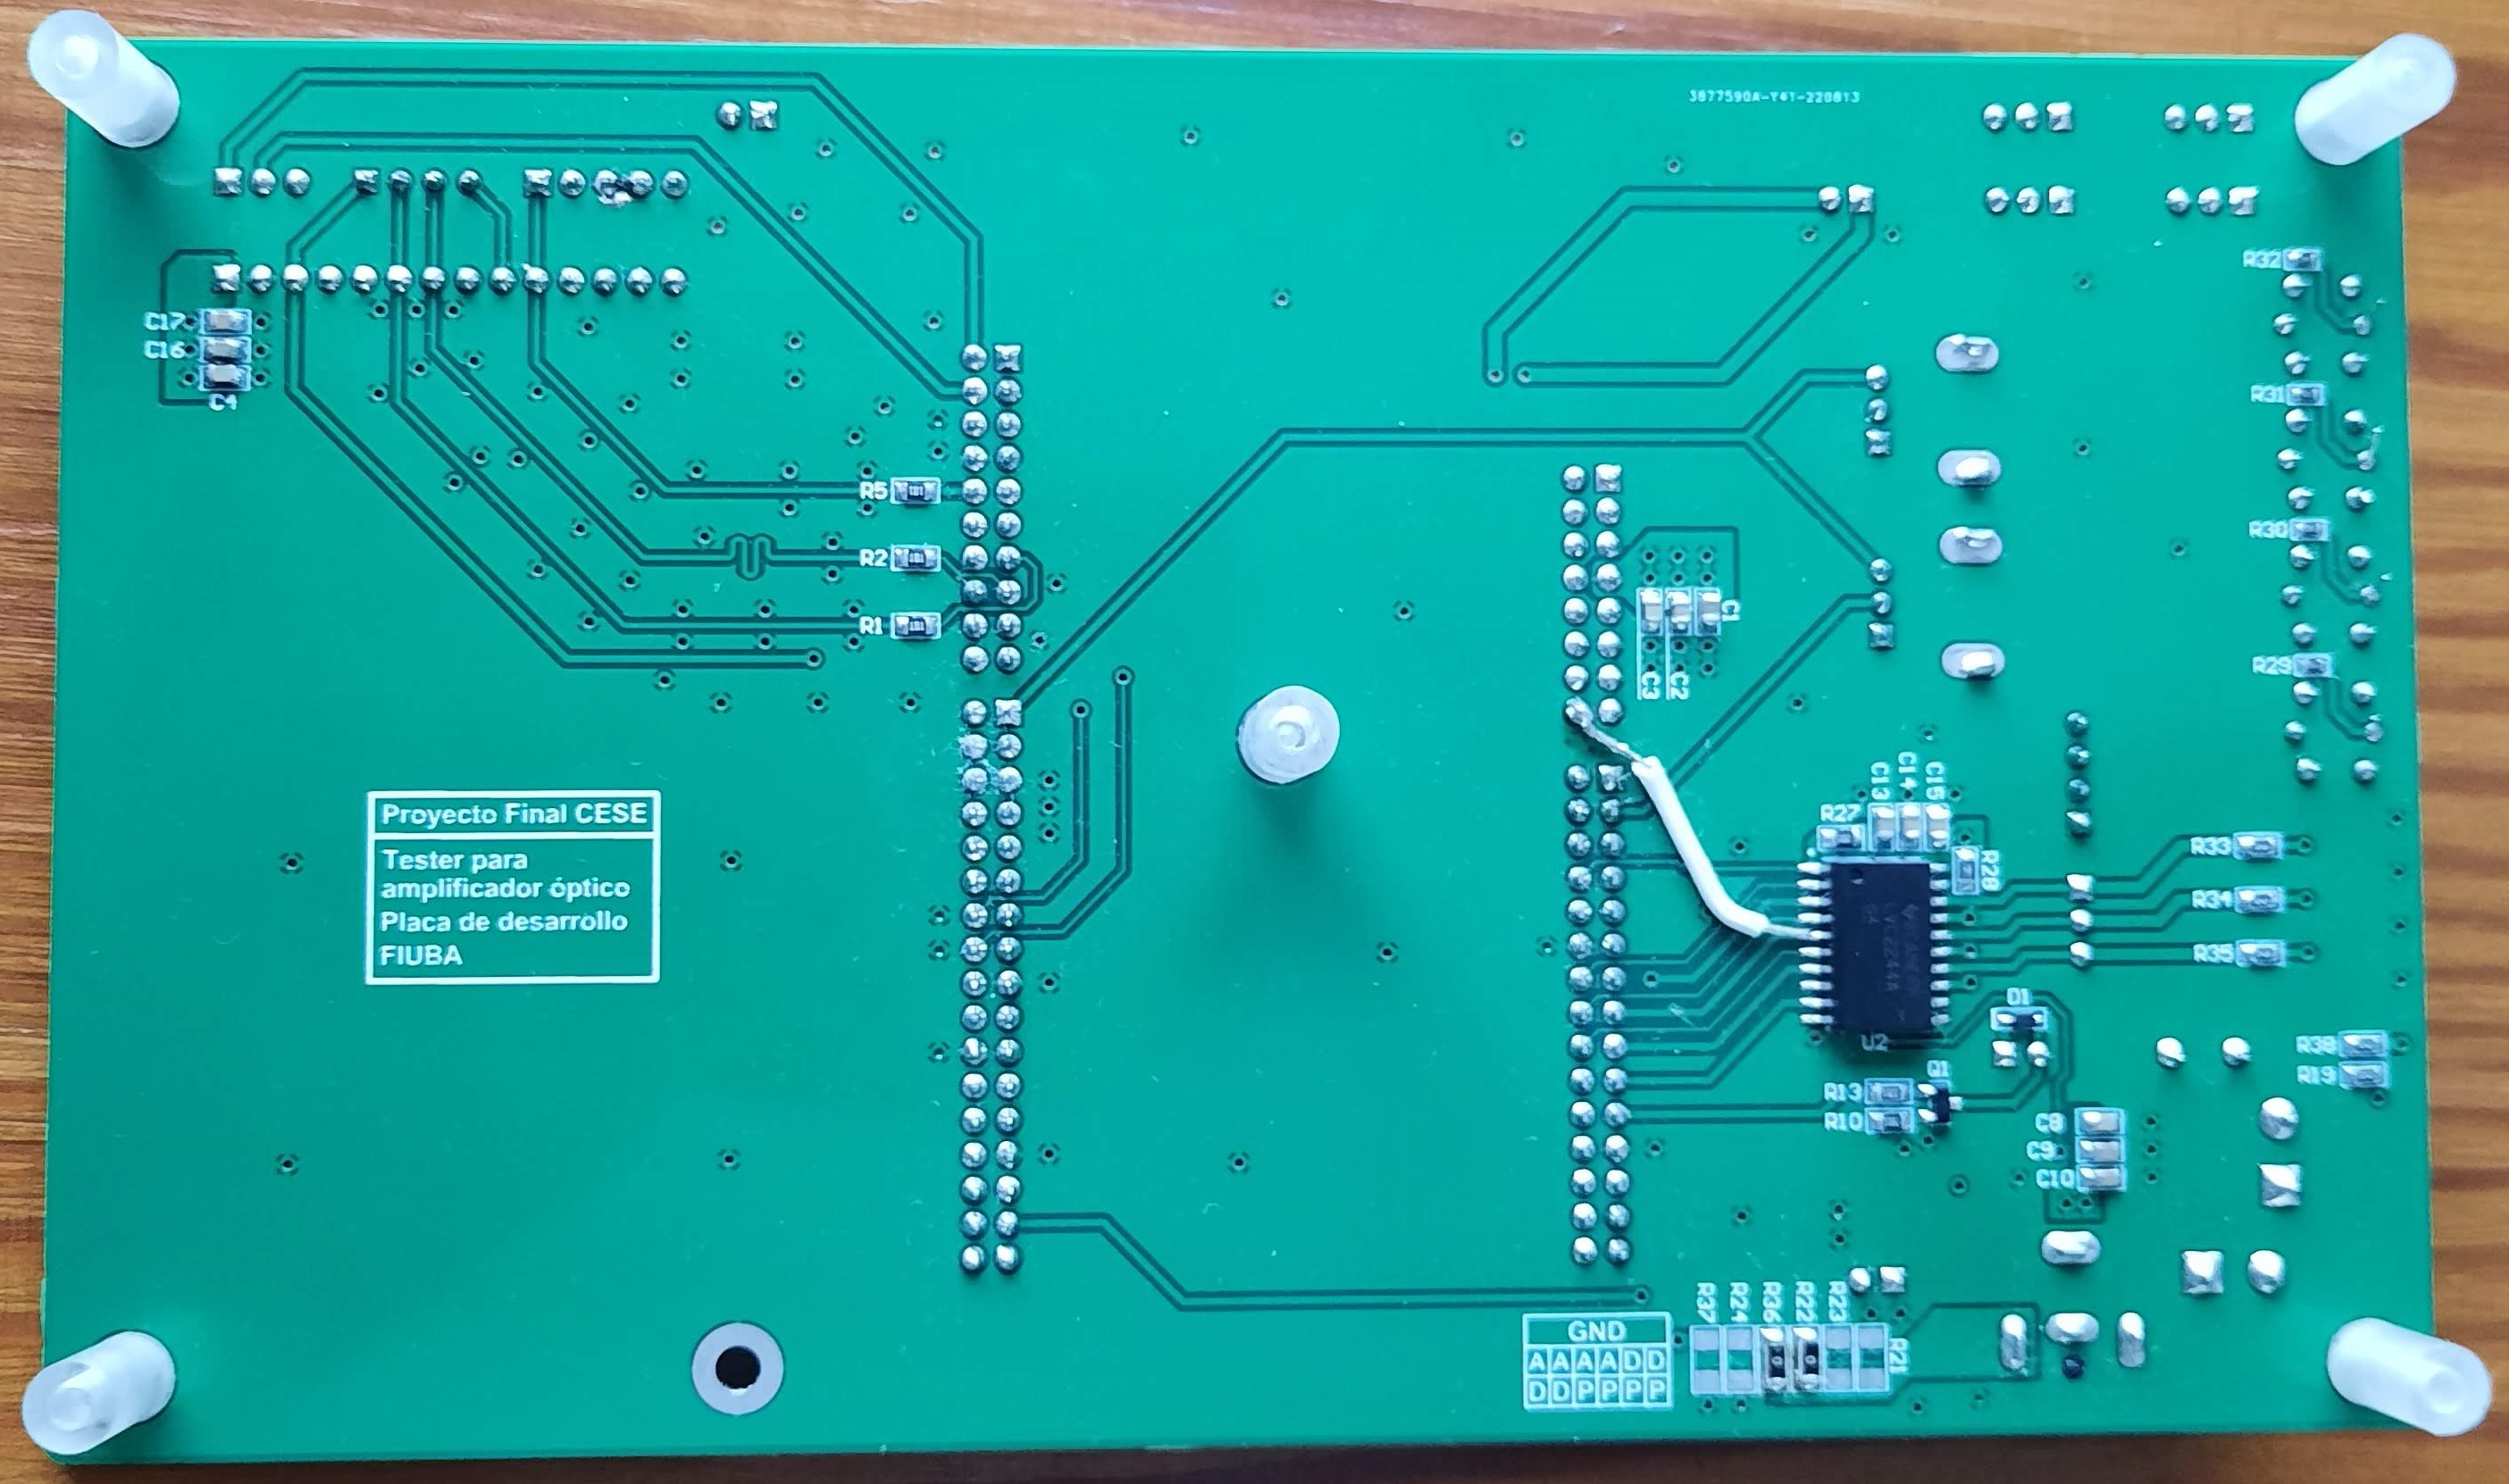
\includegraphics[width=.75\textwidth]{./Figures/placa3.jpg}
         \caption{Lado inferior del PCB.}
         \label{fig:placa2}
     \end{subfigure}
     \begin{subfigure}{\textwidth}
         \centering
         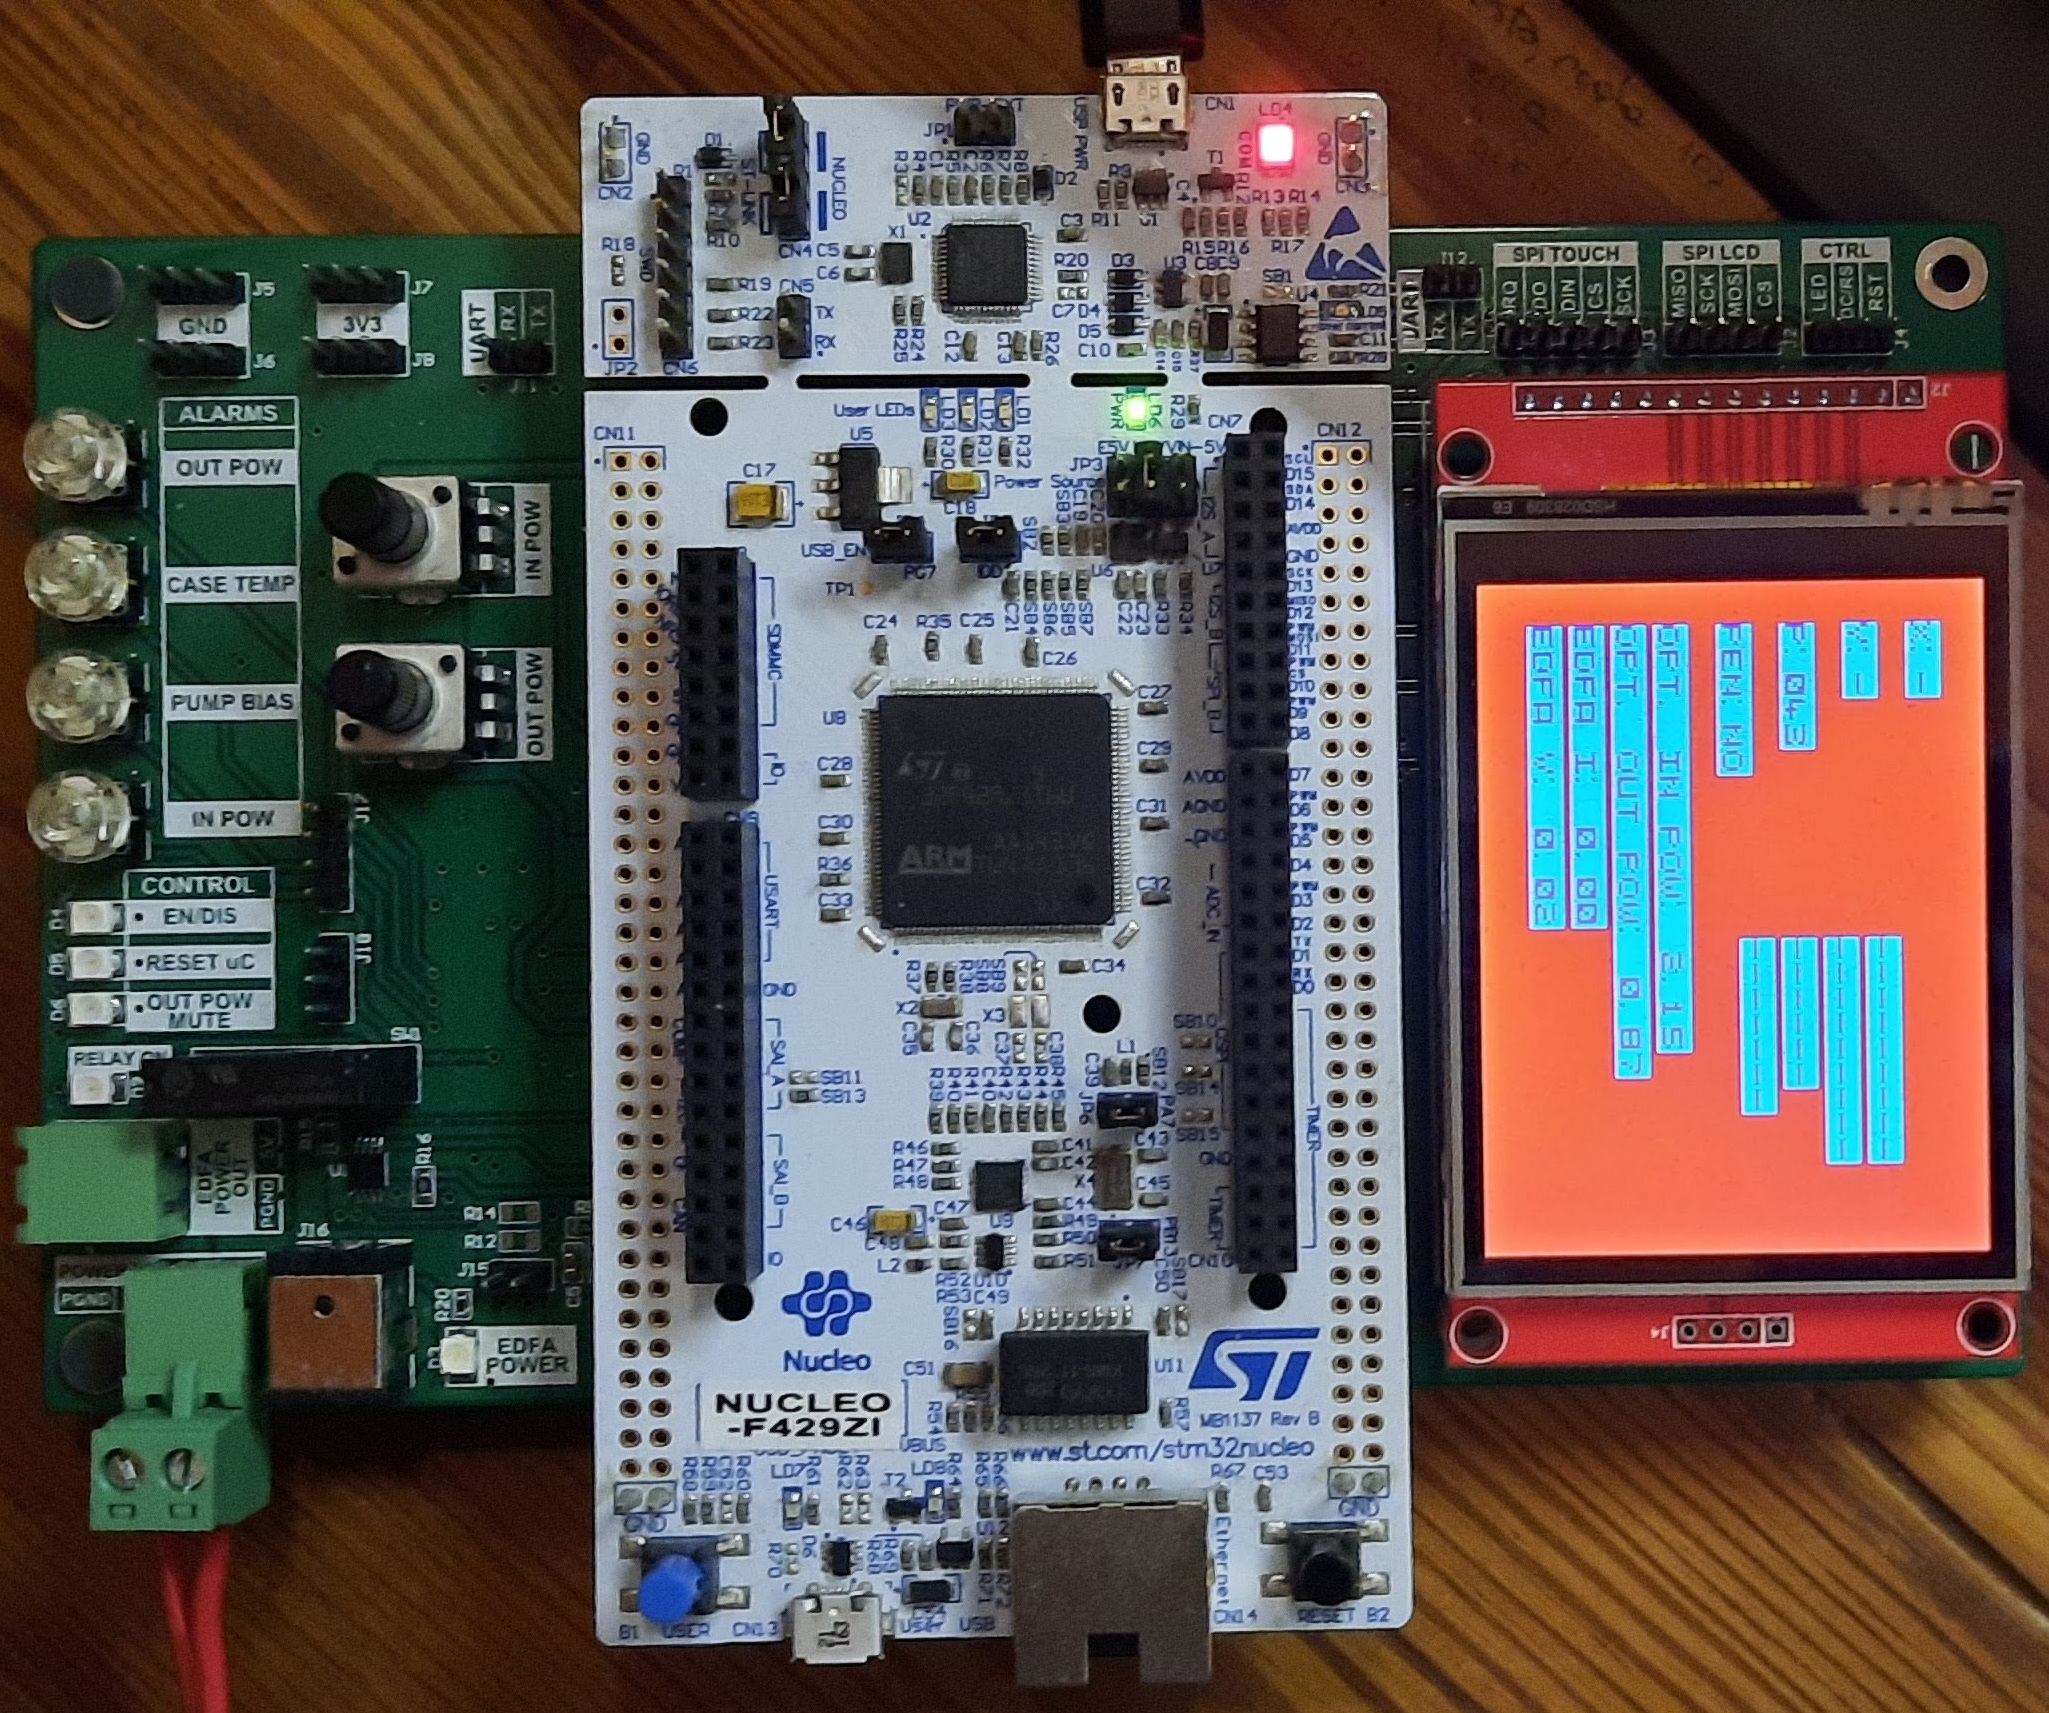
\includegraphics[width=.75\textwidth]{./Figures/placa1.jpg}
         \caption{Placa ensamblada.}
         \label{fig:placa3}
     \end{subfigure}
        \caption{Placa fabricada para el trabajo.}
        \label{fig:three graphs}
\end{figure}